\section{Surface temperature raise, numerically}
\label{sec:comsol}

The commercial software COMSOL
allows us to perform thermal simulations
with a finite-element approach.
The heat equation
to be solved
reads as
\begin{equation}
0 = \nabla(k\nabla T) + Q.
\label{eq:heateq}
\end{equation}
It is $k$ the thermal conductivity of the material
($[k]=\mathrm{m}^{-1}$),
and $Q$ the heat source
($[Q]=\mathrm{W}/\mathrm{m}^3$);
originating from the pump beam.
With this equation we take into account
only conduction
and ignore convection.
In anisotropic materials
the thermal conductivity differs
depending on the direction of conduction.
For the simulation we assume radial symmetry,
in order to bring the 3D problem down to 2D.
This saves computation time.

In this section,
I cover some numerical considerations
regarding the pump induced
temperature increase
within the different layers
of a VECSEL structure.
The presented plots
show the expected temperature profile
along the most important interface:
the top of the gain section \cite{Ranta2014OptLett}.

I only describe
the new considerations
made in the course
of this project.
While in appendix~\ref{app:comsol_deriv},
I explain
where the formulae come from
that are widely used in literature
\cite{Ranta2014OptLett,Kemp2008,Kemp2005,Vetter2012,Lindberg2005}.
This appendix also provides
additional insights,
necessary to properly implement
our structure in COMSOL.
I start by introducing
a beam profile
that was so far not considered
in these investigations.
Eventually,
I present
the calculated
pump induced temperature increase
along the surface of the gain layer
of our VECSEL structure,
considering different pump powers
and pump beam profiles.



\subsection{Pump beam profile}
\label{sec:comsol:beamprofile}

For the heat source $Q$
in (\ref{eq:heateq})
we assume
the pump beam
is incident antiparallel to the $z$-axis
(here referred to as from the top),
and of Gaussian profile.
In this orientation the heat source
associated with
each layer $j$ of the structure is given as
\cite{Kemp2008}
\begin{equation}
Q_j = \frac{2P}{\pi w^2} \eta_j\alpha_j \e^\frac{-2r^2}{w^2} \e^{-\alpha_j(z_{0j}-z)} \e^{-\sum_{i<j}\alpha_i t_i}.
\label{eq:heatsrc}
\end{equation}
This representation counts the layers
from the top down --
the sum $\sum_{i<j}$ includes the layers on top
and ignores those below the layer of interest
(in that case $j$).
A derivation,
as well as a more in-depth explanation
what the different parameters stand for,
is given in
appendix~\ref{app:comsol_deriv:Q}.

Equation (\ref{eq:heatsrc})
describes a Gaussian pump profile
by design.
In reality, however,
the pump profile is most likely not Gaussian.
In fact,
the pump spot imaged from a multimode fiber
resembles a flat-top
(also known as top-hat)
distribution \cite{Tropper2006},
or at least a super-Gaussian
\cite{Chernikov2010,Heinen2012el}.
Figure~\ref{img:visuallize_sGauss}
illustrates the difference in beam shape
of these mentioned three types.

In order to incorporate
a flat-top pump profile,
we have to replace the Gaussian part
in (\ref{eq:heatsrc}) \cite{Kemp2005}:
\begin{equation}
2\e^\frac{-2r^2}{w^2} \to
\left\{
\begin{matrix}
1 & r\leq w \\
0 & r>w.\\
\end{matrix}
\right.
\label{eq:replflattop}
\end{equation}
This can easily be verified as the renormalization has to match,
\begin{equation}
\frac{2}{w^2} \int\limits_0^\infty r \d r \e^\frac{-2r^2}{w^2}
= \frac{1}{w^2} \int\limits_0^w r \d r = \frac{1}{2}.
\label{eq:heatsrc_renorm}
\end{equation}

A super-Gaussian is of the form \cite{Chernikov2010}
\begin{equation}
f(x) \propto \e^{-|\frac{x}{w}|^\beta}.
\label{eq:super-gauss}
\end{equation}
The Gaussian profile (\ref{eq:gaussE})
corresponds to the special case $\beta=2$,
and the flat-top distribution to $\beta=\infty$.
Parameter $w$ corresponds
to the $\e^{-2}$ radius
\begin{equation}
w = \frac{\mathrm{FWHM}}{2(\frac{1}{2}\log2)^{1/\beta}}.
\end{equation}
This definition of $w$ is necessary
in order to be compatible
with the definition
of the flat-top distribution
already known in literature
\cite{Kemp2005}.
However,
in \cite{Heinen2012el}
they measured the profile
of their super-Gaussian pump,
and decided to report
the FWHM
as spot diameter.

Before we can incorporate a super-Gaussian,
we have to numerically find the normalization factor
\begin{equation}
a_p = \frac{2}{w^2} \int\limits_0^\infty r \d r \e^{-2|\frac{r}{w}|^\beta}.
\label{eq:super-gauss-scaling}
\end{equation}
Analogously to (\ref{eq:replflattop}),
for a super-Gaussian profile
we replace in (\ref{eq:heatsrc})
\begin{equation}
2\e^\frac{-2r^2}{w^2} \to \frac{1}{a_p}\e^{-2|\frac{r}{w}|^\beta}.
\label{eq:replsupergauss}
\end{equation}
Four examples for the normalization factor,
rounded to four digits, are
$a_{2}=0.5$,
$a_{3}=0.5687$,
$a_{4}=0.6267$,
and $a_\infty=0.5$.
See also
the analytic results in (\ref{eq:heatsrc_renorm}),
and Fig.~\ref{img:visuallize_sGauss}.

\begin{figure}
\centering
\subfigure{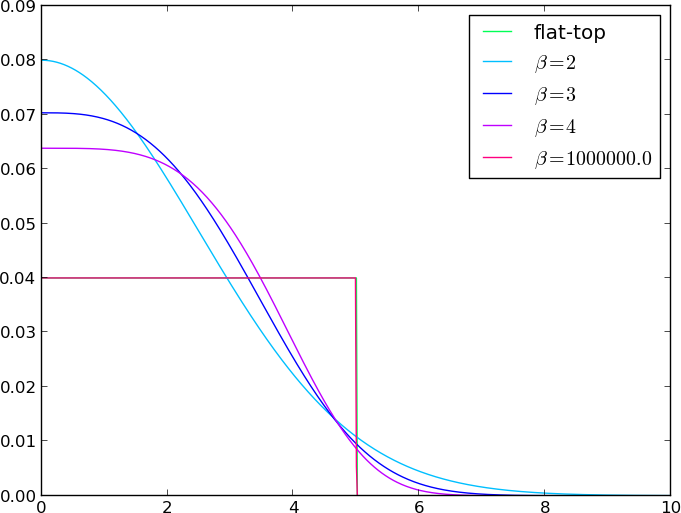
\includegraphics[width=7cm]{img/visuallize_super-Gauss_f2.png}}
\subfigure{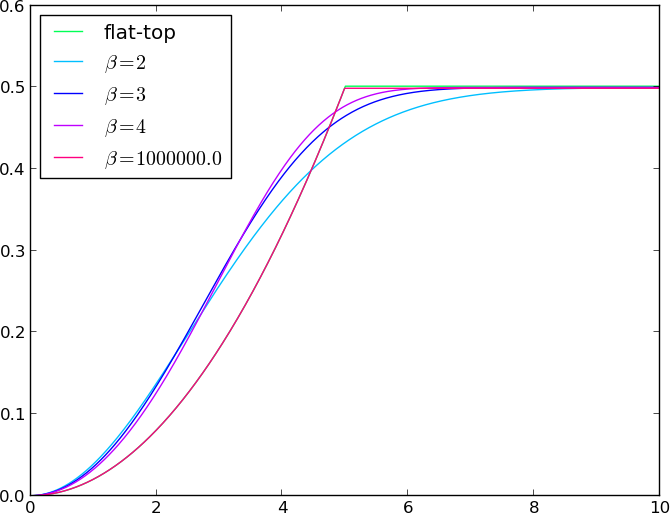
\includegraphics[width=7cm]{img/visuallize_super-Gauss_f2int.png}}
\caption{A super-Gaussian of the form
$f^2(x) \propto \e^{-2|x/w|^\beta}$
\cite{Chernikov2010}
describes an intermediate shape
between a regular Gaussian with $\beta=2$
and flat-top with $\beta=\infty$.
Left,
we see the squared shapes
of super-Gaussians $f^2(x)$ with $w=5$
for different values of $\beta$,
including flat-top as a point of reference.
The normalization is chosen such that
the over all integral corresponds to $0.5$;
from (\ref{eq:heatsrc_renorm}).
This is demonstrated in the plot to the right.}
\label{img:visuallize_sGauss}
\end{figure}
\subsection{Pump profile dependent temperature increase on gain surface}

With the concepts described in
appendix~\ref{app:comsol_deriv}
and section~\ref{sec:comsol:beamprofile}
we can look at
the expected temperature increase
of our structure,
corresponding to different pump beam profiles.
The thermal load
inflicted on the structure
depends on this pump distribution.
The image of a multi-mode fiber
can be described by a super-Gaussian.
This category describes
a generalized Gaussian profile
of the form $f(x)\sim\e^{-|\frac{x}{w}|^\beta}$
\cite{Chernikov2010},
see Fig.~\ref{img:visuallize_sGauss}.
It covers
distributions between
Gaussian ($\beta=2$) and flat-top ($\beta=\infty$).
The closer the pump beam distribution
resembles a flat-top distribution,
the more evenly the temperature load
is distributed.

The numerical analysis
for super-Gaussian profiles
is particularly interesting:
while the temperature profile
caused by Gaussian and flat-top distributions
were already reported \cite{Kemp2005},
the intermediate super-Gaussian profile
was ignored thus far.
The fact that
the pump profile
is relevant
for the performance of VECSELs
was demonstrated in \cite{Chernikov2010}.

We can assume roll over occurs
once the gain material exceeds
a critical temperature \cite{Heinen2012},
see section~\ref{sec:rth}.
In order to postpone
the critical pump power
to higher values,
we have to lower the peak temperature
invoked by the pump.
Figure~\ref{img:Comsol_Tvsr} shows,
this can be achieved
by either assuming
a super-Gaussian beam profile
or a regular Gaussian
with larger spot size.

\begin{figure}
\centering
\subfigure{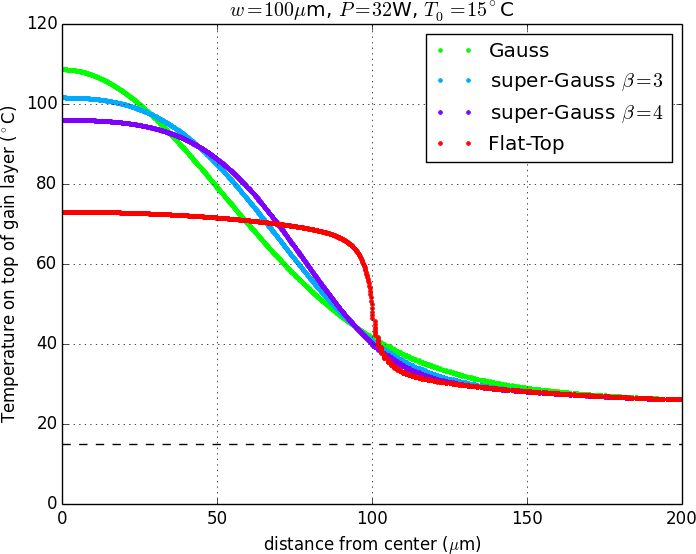
\includegraphics[width=7cm]{img/Comsol_Tvsr_32W_100um.png}}
\subfigure{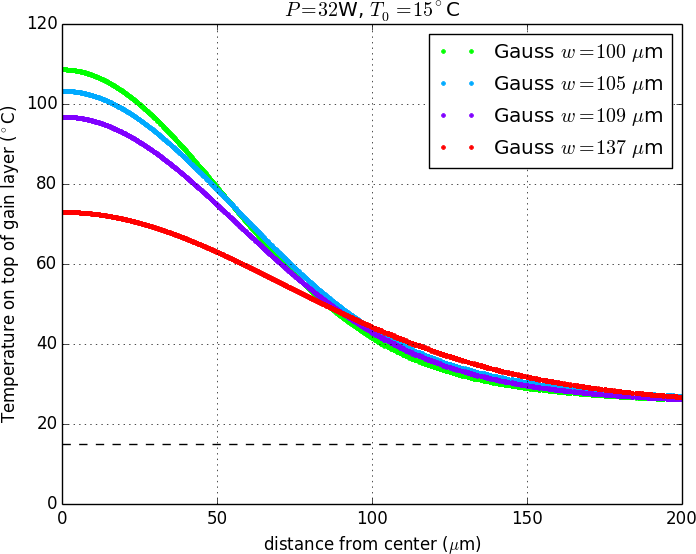
\includegraphics[width=7cm]{img/Comsol_Tvsr_32W_sG-equivs.png}}
\caption{Temperature along surface of the gain section, $z_\mathrm{0g}$
(Tab.~\ref{tab:comsolparams}).
The different beam shapes from Fig.~\ref{img:visuallize_sGauss}
with the same total power
induce a different increase in temperature
with respect to $T_0$,
indicated by the dashed line (left).
The same peak temperature can be found
employing regular Gaussians
with larger beam spots.
These however,
have a larger fraction
of the power distribution
below threshold
in the tail region,
which contributes only to heating
but no light emission.}
\label{img:Comsol_Tvsr}
\end{figure}

The peak temperature
is not the only relevant quantity
for an efficient pump profile:
the gain needs to be irradiated
with enough power
to transcend threshold.
The regions of the sample
irradiated by pump light
but below threshold
do not contribute to the laser output.
However, these regions do heat the structure.

The stronger we pump,
the larger the area on the sample
irradiated by above-threshold power.
This above-threshold
region corresponds to
the relevant, effective area.
In the case of the accentuated Gaussian beam,
the center exceeds
the roll over temperature
at a relatively low pump power,
while the effective area
is still relatively small.
In contrast,
a super-Gaussian pump profile
is capable activating
a larger effective area,
while at the same time
lowering the peak temperature.
Consequentially,
roll over is expected
to occur at higher pump power.

These simulations demonstrate
the thermal management
depends on the pump profile.
Furthermore, they suggest
a Gaussian pump profile
to be non-ideal
concerning the inflicted thermal load.
This reasoning is consistent
with the findings in \cite{Chernikov2010}.

This provokes
me to issue a warning:
extracting thermal resistance $\Rth$
only for the hottest spot,
as suggested in section~\ref{sec:rth},
does not tell the full story.
We can find normal Gaussians
with the same peak temperature
as super-Gaussians,
Fig.~\ref{img:Comsol_Tmax_BeamProfile}.
Comparing thus extracted values of $\Rth$
with values measured with other setups --
and expectedly different pump profiles --
is hence not valid.

\begin{figure}
\centering
\subfigure{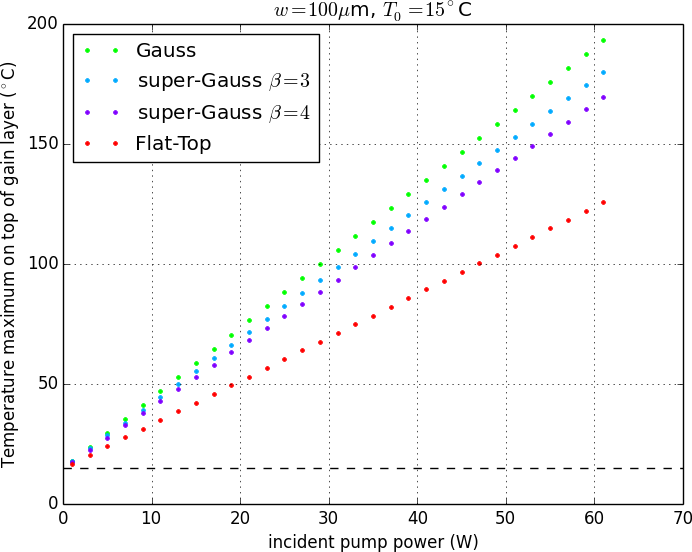
\includegraphics[width=7cm]{img/Comsol_Tmax_BeamProfile_32W_100um.png}}
\subfigure{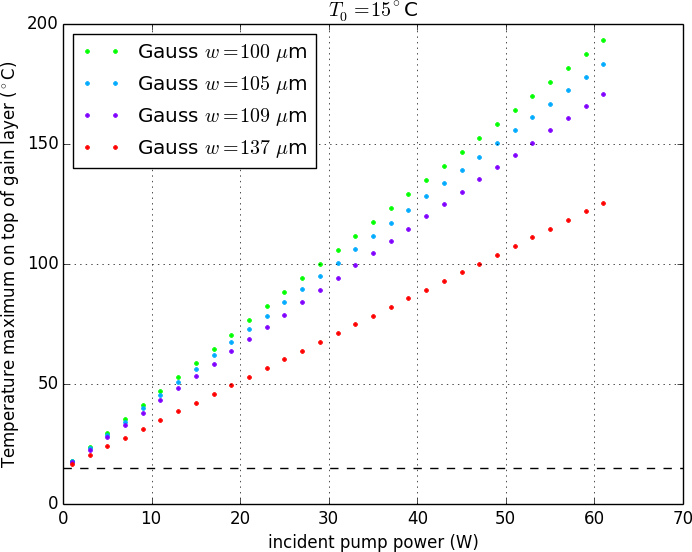
\includegraphics[width=7cm]{img/Comsol_Tmax_BeamProfile_32W_sG-equiv.png}}
\caption{The maximum temperature (i.e. at $r=0\,\mu\mathrm{m}$)
of the different beam profile depicted in Fig.~\ref{img:Comsol_Tvsr},
for various settings of total power.
The increase in peak temperature
does not change qualitatively
whether we consider super-Gaussians (left)
or regular Gaussians with larger radii (right).}
\label{img:Comsol_Tmax_BeamProfile}
\end{figure}




